\documentclass[10pt,a4paper]{article}
\usepackage[utf8]{inputenc}
\usepackage[francais]{babel}
\usepackage[T1]{fontenc}
\usepackage{hyperref}
\usepackage{eurosym}
\usepackage{listings}
\usepackage{color}
\usepackage{graphicx}
\usepackage[titletoc,toc,title]{appendix}
\usepackage{fullpage}

\author{Anthony \textsc{Caccia} \and Romain \textsc{Fontaine} \and Nikita \textsc{Marchant} }
\date{}
\title{\textsc{INFO-F-309 : Administration Système} Projet : Rapport d'implémentation}

\setlength{\parindent}{1.5em}
\setlength{\parskip}{1em}
% \renewcommand{\baselinestretch}{1.5}

\lstset{%
    inputencoding=utf8,
    extendedchars=true,
    commentstyle=\color{red},
    keywordstyle=\color{blue},
    literate=%
            {é}{{\'{e}}}1
            {è}{{\`{e}}}1
            {ê}{{\^{e}}}1
            {ë}{{\¨{e}}}1
            {û}{{\^{u}}}1
            {ù}{{\`{u}}}1
            {â}{{\^{a}}}1
            {à}{{\`{a}}}1
            {î}{{\^{i}}}1
            {ô}{{\^{o}}}1
            {ç}{{\c{c}}}1
            {Ç}{{\c{C}}}1
            {É}{{\'{E}}}1
            {Ê}{{\^{E}}}1
            {À}{{\`{A}}}1
            {Â}{{\^{A}}}1
            {Î}{{\^{I}}}1
}
\begin{document}
\maketitle

\tableofcontents
\newpage

\section{Introduction}
\label{sec:Introduction}

Le but de ce projet est de permettre à nos clients la compilation en ligne de documents rédigés au format \LaTeX sur un serveur distant.

Pour cela, une interface web sera mise en place afin de téléverser une archive contenant les sources du document à compiler.
Puis, à la réception de ce document, le serveur enverra les sources dans une BSDJail afin qu'elles soient traitées sans posssibilité de compromission de celui-ci.

\section{Machines déployées}
\label{sec:Machines déployées}

Deux machines ont été déployées: une première machine sur laquelle tourne la distribution GNU/Linux Debian, et une deuxième qui a pour système d'exploitation la distribution FreeBSD.

La première machine a pour tâche la mise en service de l'interface web
(voir les figures \ref{app1} et \ref{app2}),
le stockage des fichiers \texttt{zip} et \texttt{pdf}
ainsi que l'envoi des ordres de compilation sur la seconde machine.

La seconde machine reçoit les ordres de compilation, crée des BSDJails à la volée, y place les sources récupérées sur la première machine,
y lance les compilations et l'analyse antivirus et renvoie le document pdf final à la première machine.

\begin{figure}[h]
   \centering
   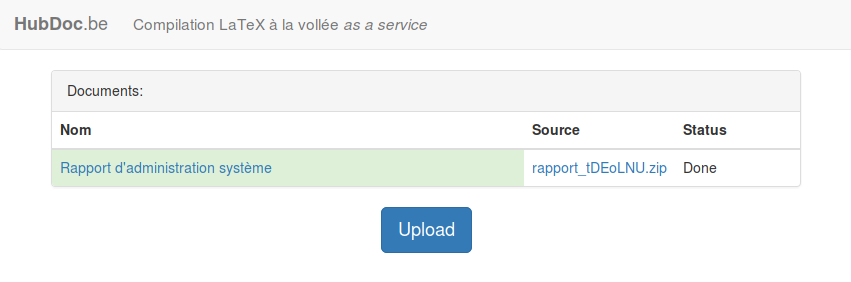
\includegraphics[scale=0.4]{hubdoc.png}
   \caption{\label{app1} Application web - Page d'accueil}
\end{figure}

\begin{figure}[!h]
   \centering
   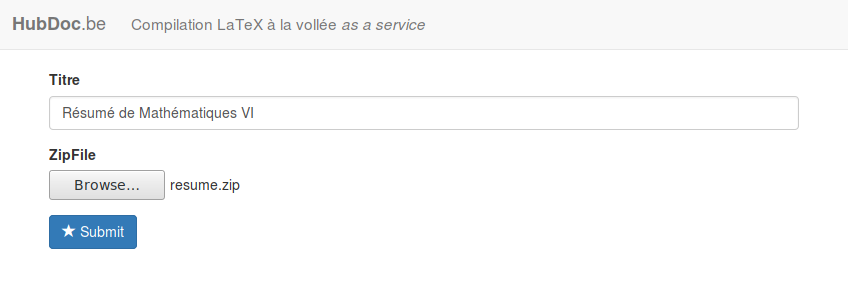
\includegraphics[scale=0.4]{hubdoc-upload.png}
   \caption{\label{app2} Application web - Page de téléversement}
\end{figure}

\section{Serveur web (Machine Debian)}
\subsection{Services}
Les services suivants tournent sur le premier serveur :

\texttt{Nginx} : il sert de proxy http pour l'application \texttt{Django} et sert via http les fichiers \texttt{zip} et \texttt{pdf}.
Il écoute sur toutes les interfaces et sur le port \texttt{80}.
Commande : \texttt{systemctl start/stop/status nginx.service}

\texttt{Postgresql} : le serveur de base de données.
Il sert une unique base de données : \texttt{webview} qui est utilisée par l'application web.
Il écoute en local sur un socket UNIX ansi que sur l'interface publique (retreinte par le firewall) sur le port \texttt{5432}.
Commande : \texttt{systemctl start/stop/status nginx.service}

\texttt{Redis} est utilisé comme message broker entre \texttt{Celery} et l'application web.
Celui-ci écoute sur toutes les interfaces (l'interface publique est restreinte par le firewall) sur le port \texttt{6379} et demande un mot de passe.
Commande : \texttt{systemctl start/stop/status redis-server.service}

\texttt{Django} : C'est un processus \texttt{gunicorn} qui sert l'application web sur le port \texttt{8000} sur \texttt{localhost}.
Commande : \texttt{systemctl start/stop/status django.service}

Serveur \texttt{nfs} : le répertoire \texttt{/var/nfs} est partagé avec la machine BSD via \texttt{nfs}.
Dans celui-ci se trouve \texttt{/var/nfs/webview/media} dans lequel sont stockés tous les fichiers media de Django (principalement les fichiers \texttt{zip} et \texttt{pdf}).
Commande : \texttt{systemctl start/stop/status nfs-kernel-server.service}

\texttt{NTP} : vu que nous travaillons sur plusieurs machines en parralèlle, il est indispensable d'avoir la même heure partout.
C'est le travail de \texttt{NTP}.
Commande : \texttt{systemctl start/stop/status ntp.service}

\texttt{iptables} : il sert de firewall pour les différents services qui écoutent sur l'interface publique.
Il protège le serveur Redis et le serveur Postgresql en limitant les connexions à celles venant de l'ip de la machine bsd.
Les commandes à utiliser pour ajouter des nouvelles règles sont \texttt{iptables} et \texttt{ip6tables}.
Après cela, on utilise \texttt{iptables-persistent} pour conserver les règles après chaque reboot. Pour se faire il suffit d'exécuter \texttt{iptables-save > /etc/iptables/rules.v4} et \texttt{ip6tables-save > /etc/iptables/rules.v6}.


\subsection{Procédure d'installation}

Premièrement, il faut installer tous les paquets dont nous avons besoin :
\begin{lstlisting}[language=bash]
  apt-get update
  apt-get install git sudo zsh nginx \
    nfs-kernel-server vim redis-server postgresql-server \
    python3 python3-dev ntpdate ntp screen iptables-persistent
\end{lstlisting}

\subsubsection{\texttt{nfs}}

Nous avons choisi de partager \texttt{/var/nfs}. Pour cela, il faut le créer et lui donner les bonnes permissions :

\begin{lstlisting}[language=bash]
  mkdir /var/nfs
  chown nobody:nogroup /var/nfs
\end{lstlisting}

Ensuite il faut éditer \texttt{/etc/exports} (\ref{subs:etc-exports}) puis y ajouter le chemin vers
le dossier ainsi que les ip des machines autorisées à s'y connecter.

Après avoir édité ce fichier, il faut prévenir le daemon qu'il a changé et démarrer le serveur :
\begin{lstlisting}[language=bash]
  exportfs -a
  systemctl enable nfs-kernel-server
  systemctl start nfs-kernel-server
\end{lstlisting}

Pour terminer il faut créer le dossier dans lequel se trouveront les fichiers à partager et lui donner les bonnes permissions :
\begin{lstlisting}[language=bash]
  mkdir -p /var/nfs/webview/media
  chown www-data:www-data /var/nfs/webview/
\end{lstlisting}

\subsubsection{\texttt{nginx}}

Nous devons créer un virtualhost \texttt{nginx} pour reverse-proxifier \texttt{gunicorn}.
Il faut éditer \\\texttt{/etc/nginx/sites-available/hubdoc.be} comme dans l'annexe (\ref{subs:deb-nginx-sites-avail-hubdoc})
puis créer un lien symbolique dans \texttt{sites-enabled} pour l'activer et pour finir,
recharger la configuration :
\begin{lstlisting}[language=bash]
  ln -s /etc/nginx/sites-available/hubdoc.be /etc/nginx/sites-enabled/
  systemctl reload nginx
\end{lstlisting}

\subsubsection{\texttt{redis}}

Vu que qu'il sera accessible de l'extérieur,
il faut demander à \texttt{redis} d'exiger un mot de passe.
Pour cela, editez \texttt{/etc/redis/redis.conf} et décommentez \texttt{requirepass}
et changez le mot de passe qui est à côté.

Il faut aussi lui demander d'écouter sur toutes les interfaces.
Pour cela, remplacez \texttt{bind 127.0.0.1} par \texttt{bind 0.0.0.0}.

Pour finir, redémarrez le service : \texttt{systemctl restart redis-server.service}


\subsubsection{\texttt{postgesql}}

Il faut autoriser la machine bsd à se connecter à \texttt{postgesql}.
Pour cela, il faut éditer \\\texttt{/etc/postgresql/9.4/main/pg\_hba.conf} (\ref{subs:deb-pg-hba}) et rajouter :
\begin{lstlisting}[language=bash]
  host  all  all 146.185.151.186/32  md5
\end{lstlisting}
En dessous de la ligne
\begin{lstlisting}[language=bash]
  host  all  all 127.0.0.1/32        md5
\end{lstlisting}

Ensuite il faut demander à \texttt{postgesql} d'écouter sur toutes les interfaces :
Dans \\\texttt{/etc/postgresql/9.4/main/postgresql.conf}, changez
\begin{lstlisting}[language=bash]
  #listen_addresses = 'localhost'
\end{lstlisting}
par
\begin{lstlisting}[language=bash]
  listen_addresses = '*'
\end{lstlisting}

Puis redémarrez le service : \texttt{systemctl restart postgresql}.

\texttt{Django} a besoin d'une base de données.
Pour la créer, il faut exécuter en tant que \texttt{postgres} :
\begin{lstlisting}[language=bash]
  createuser -P www-data # assignez un mot de passe à l'utilisteur
  createdb -O www-data webbview
\end{lstlisting}

\subsubsection{\texttt{iptables}}
Pour éviter d'avoir nos services accessible par tout le monde, nous utilisons iptables comme firewall.
Pour ce faire, nous utilisons les commandes suivantes
(\texttt{146.185.151.186} étant l'ip de la machine bsd):


Pour \texttt{Redis}:
\begin{lstlisting}[language=bash]
  iptables -A INPUT -p tcp --destination-port 6379 -j DROP
  ip6tables -A INPUT -p tcp --destination-port 6379 -j DROP
  iptables -I INPUT -p tcp -s 127.0.0.1 --dport 6379 -j ACCEPT
  iptables -I INPUT -p tcp -s 146.185.151.186 --dport 6379 -j ACCEPT
\end{lstlisting}

Pour \texttt{Postgresql}:
\begin{lstlisting}[language=bash]
  iptables -A INPUT -p tcp --destination-port 5432 -j DROP
  ip6tables -A INPUT -p tcp --destination-port 5432 -j DROP
  iptables -I INPUT -p tcp -s 127.0.0.1 --dport 5432 -j ACCEPT
  iptables -I INPUT -p tcp -s 146.185.151.186 --dport 5432 -j ACCEPT
\end{lstlisting}

Et pour garder de la persistance après chaque redémarrage:
\begin{lstlisting}[language=bash]
  iptables-save > /etc/iptables/rules.v4
  ip6tables-save > /etc/iptables/rules.v6
\end{lstlisting}

\subsubsection{\texttt{Django}}

Il faut, en tant que \texttt{www-data}, récupérer les sources de l'application et installer les dépendances :
\begin{lstlisting}[language=bash]
  cd /var/www
  git clone https://github.com/C4ptainCrunch/info-f-309.git
  cd info-f-309/webview
  virtualenv ve
  source ve/bin/activate
  pip install -r requirements.txt
  pip install psycopg2
\end{lstlisting}

Ensuite il faut configurer l'application avec le fichier\\
\texttt{/var/www/info-f-309/webview/local\_settings.py}
(voir \ref{fichier-annexe-local-settings})

Après, on peut collecter les fichiers statiques et remplir la base de données :
\begin{lstlisting}[language=bash]
  ./manage.py collectstatic
  ./manage.py migrate
\end{lstlisting}

Pour finir, il faut installer pui démarrer le service \texttt{systemd} :
déposez le fichier \ref{subs:deb-django-service} dans \\\texttt{/etc/systemd/system/django.service} puis exécutez :
\begin{lstlisting}[language=bash]
  systemctl daemon-reload
  systemctl enable django
  systemctl start django
\end{lstlisting}


\subsection{Mise à jour}

Dans le cas ou l'on voudrait mettre à jour ce serveur,
il faut exéccuter ces deux commandes en tant que root :
\texttt{apt-get update}, \texttt{apt-get upgrade}.

Pour mettre à jour l'application web, en tant que \texttt{www-data}
il faut exécuter \texttt{git pull} depuis le dossier \texttt{/var/www/info-f-309}
et ensuite en tant que \texttt{root} exécuter \texttt{systemctl restart django}.

Dans le cas ou le schéma de la base de donnée aurait changé,
il faut aussi exécuter \\\texttt{/var/www/info-309/webview/ve/bin/python /var/www/info-309/webview/manage.py migrate} depuis l'utilisateur \texttt{www-data}.

\section{Serveur de compilation (Machine BSD)}
\subsection{Services}

\texttt{Celery} : Celery est un ``worker'' : il écoute sur le ``message broker'' (le \texttt{redis} qui tourne sur l'autre machine) en attendant des ordres.
Dès qu'il recoit une tache, il l'exécute et renvoie le résultat au ``message broker''.
C'est \texttt{Celery} qui récupérera les fichiers sur le \texttt{nfs}, créera une \texttt{jail}, y compilera le \LaTeX, etc.
Commande : \texttt{service celery start/stop}

\texttt{ClamAV} : c'est l'outil qui nous permet de détecter des signatures de virus dans les pdf.
Celui-ci est découpé en deux daemons :
        \begin{itemize}
            \item \texttt{clamd} : le processus qui vérifie les fichiers.

            Il est accessible depuis \texttt{unix://var/run/clamav/clamd.sock}

            (Commande : \texttt{/usr/local/etc/rc.d/clamav-clamd start/stop})
            \item \texttt{freshclam} s'occupe de garder la base de signatures à jour.

            (Commande : \texttt{/usr/local/etc/rc.d/clamav-freshclam start/stop})
        \end{itemize}

\vspace{1em} % wtf latex
Client \texttt{nfs} : il se connecte à la machine Debian et permet à \texttt{Celery} d'avoir accès aux fichiers téléversés sur l'autre machine ainsi qu'à renvoyer les fichiers compilés.
Commande : \texttt{service nfsclient start/stop} ainsi que \texttt{mount /mnt} et \texttt{umount /mnt}.

\texttt{NTP} : même utilité que sur l'autre machine.
Commande : \texttt{service start/stop ntpd}.

\subsection{Installation}
Pour commencer, il a fallu installer les paquets dont nous dépendons avec la commande \emph{pkg}:
\begin{lstlisting}[language=bash]
  pkg update
  pkg install bash zsh mosh git nginx python34 vim subversion
  pkg install cpdup py34-sqlite3 py27-psycopg2 clamav
\end{lstlisting}

\subsection{Contrôle des BSDJails}
\label{subs:Contrôle des BSDJails}
Afin de pouvoir créer des BSDJails, il nous faut d'abord construire un espace utilisateur de référence.
Il nous faut pour cela mettre à jour les sources FreeBSD situées dans le dossier \texttt{/usr/src}:
\begin{lstlisting}[language=bash]
  freebsd-update fetch
  freebsd-update install
\end{lstlisting}

On peut ensuite supprimer l'éventuel ancien build, en n'oubliant pas de modifier les flags des fichiers pour que ceux-ci puissent être modifiés :
\begin{lstlisting}[language=bash]
  chflags -R noschg /usr/obj
  rm -rf /usr/obj
\end{lstlisting}

Afin de minimiser la taille du build, il peut être construit en omettant certaines parties du filesystem. Il suffit pour cela d'éditer le fichier \texttt{/etc/src.conf} (voir \ref{sub:etc-src-conf}).
Enfin, on peut lancer la compilation de ce build, ce qui peut prendre un certain temps (plus de deux heures en général):
\begin{lstlisting}[language=bash]
  cd /usr/src
  make buidworld
\end{lstlisting}

À partir de ce build, il a été décidé de créer un modèle pour la création des jails.
Ce modèle sera en deux parties:
\begin{itemize}
  \item la première partie située dans \texttt{/home/j/mroot} qui contiendra la partie commune à toutes ces jails, et qui sera toujours en lecture seule,
  \item la seconde partie située dans \texttt{/home/j/skel} qui contiendra des dossiers propres à chaque jail et qui seront accessible en lecture-écriture.
\end{itemize}

Pour commencer, la première partie va être créée grâce à ces deux commandes:
\begin{lstlisting}[language=bash]
  cd /usr/src
  mkdir /home/j/mroot
  # crée un "sous-système" dans le dossier DESTDIR
  make installworld DESTDIR=/home/j/mroot
  # copie les fichiers de configuration dans la jail
  make distribution DESTDIR=/home/j/mroot
\end{lstlisting}

Là, le dossier dans \texttt{DESTDIR} contiendra un sous-système dans lequel nous pouvons installer les logiciels nécessaires aux tâches de ces jails, c'est à dire la compilation \LaTeX:
\begin{lstlisting}[language=bash]
  chroot /home/j/mroot   # installation des logiciels nécessaires
  pkg update && pkg install texlive-full
  exit
\end{lstlisting}

Ensuite, nous allons déplacer les dossiers accessibles en lecture-écriture dans la seconde partie et ajouter des liens symboliques dans le dossier \texttt{/home/j/mroot/s}, où sera monté celle-ci:
\begin{lstlisting}[language=bash]
  mkdir /home/j/skel
  mv /home/j/mroot/etc /home/j/skel
  mv /home/j/mroot/root /home/j/skel
  mv /home/j/mroot/tmp /home/j/skel
  mv /home/j/mroot/home /home/j/skel
  cd /home/j/mroot
  mkdir s
  ln -s s/etc etc
  ln -s s/root root
  ln -s s/home home
  ln -s s/tmp tmp
\end{lstlisting}
Nous avons dès lors notre modèle pour la création de jails.

Voici maintenant un exemple de création d'une jail, nommée example.
On commence par créer les dossiers contenant la jail, le premier simplement avec \texttt{mkdir},
le deuxième avec la commande \texttt{cpdup}, qui crée une exacte réplique du fichier source.
On peut ensuite les monter grâce aux commandes \texttt{mount\_nullfs} et \texttt{mount}.
Cette première commande permet d'accéder à des fichiers depuis différents emplacements.

\begin{lstlisting}[language=bash]
  mkdir /home/j/example
  cpdup /home/j/skel /home/js/example
  mount_nullfs -o ro /home/j/mroot /home/j/example
  mount_nullfs -o rw /home/js/example /home/j/example/s
  mount -t devfs /dev /home/j/example/dev
\end{lstlisting}
Là, on peut utiliser la commande \texttt{jail} afin de lancer une jail:
\begin{lstlisting}[language=bash]
  jail -c path=/home/j/example name=example persist
\end{lstlisting}
\texttt{-c} indique que l'on crée une jail, \texttt{path} indique l'emplacement de la jail,
\texttt{name} son nom et l'option \texttt{persist} garde la jail en route même si celle-ci n'accomplit aucune action.

Afin d'accéder à cette jail depuis l'extérieur, il suffit d'accéder à l'emplacement où celle-ci se situe.
Pour lancer une commande à l'intérieur de cette jail,
on utilise la commande \texttt{jexec} dont le premier argument est soit le nom de la jail,
soit son jid (qui peut être déterminé grâce à la commande \texttt{jls}),
et les autres arguments correspondent à la commande à exécuter.
Par exemple, pour ajouter un fichier \texttt{test.txt} dans la jail depuis l'extérieur et le lister depuis l'intérieur:
\begin{lstlisting}[language=bash]
  touch /home/js/example/home/test.txt
  jexec example ls /home
\end{lstlisting}

Pour désactiver et supprimer cette jail, il faut tout d'abord la stopper grâce à la commande \texttt{jail} à laquelle on passe le flag \texttt{-r}.
Puis on démonte tous les dossiers montés et on peut enfin les supprimer.
\begin{lstlisting}[language=bash]
  jail -r example
  umount /home/j/example/s
  umount /home/j/example/dev
  umount /home/j/example
  chflags -R noschg /home/j/example
  chflags -R noschg /home/js/example
  rm -rf /home/j/example
  rm -rf /home/js/example
\end{lstlisting}

\subsection{Configuration du NFS}
\begin{enumerate}
  \item ajouter \texttt{nfs\_client\_enable="YES"} dans \texttt{/etc/rc.conf} (\ref{subs:etc-rc-conf})
  \item démarrer le service avec \texttt{service nfsclient start}
  \item ajouter la ligne \texttt{192.81.220.4:/var/nfs        /mnt        nfs        rw        0        0} à \texttt{/etc/fstab} (\ref{subs:etc-fstab})
  \item remonter le sytème de fichier défini dans le fstab avec \texttt{mount -a}
\end{enumerate}

\subsection{Configuration du NTP}
\begin{enumerate}
  \item ajouter \texttt{ntpd\_enable="YES"} dans \texttt{/etc/rc.conf} (\ref{subs:etc-rc-conf})
  \item démarrer le service avec \texttt{service ntpd start}
\end{enumerate}

\subsection{Configuration de Celery}
On commence par créer un user \texttt{celery} avec la commande interactive \texttt{adduser}:
\begin{description}
  \item[Username] celery
  \item[Full name] celery
  \item[Shell] bash
  \item[Use password-based authentication?] no
\end{description}

Celery sera installé dans un environnement virtuel python, nous devons donc nous assurer de disposer des paquets pip et virtualenv:
\begin{lstlisting}[language=bash]
  sudo python3.4 -m ensurepip # installe pip pour python3.4
  sudo python3.4 -m pip install virtualenv # install virtualenv
\end{lstlisting}

Il faut ensuite créer des dossiers pour sauvegarder les pid et les logs de Celery:
\begin{lstlisting}[language=bash]
  sudo mkdir /var/log/celery
  sudo chown celery:celery /var/log/celery/
  sudo mkdir /var/run/celery
  sudo chown celery:celery /var/run/celery/
\end{lstlisting}

Les sources du programme étant sur le site d'hébergement Github, l'user celery va cloner le dépôt dans sa home, initialiser un virtualenv et installer les dépendances.
\begin{lstlisting}[language=bash]
  su celery
  cd      # retourner dans la home de celery
  git clone https://github.com/C4ptainCrunch/info-f-309.git
  cd info-f-309/webview
  virtualenv ve
  source ve/bin/activate
  pip install -r requirements.txt
  pip install psycopg2
\end{lstlisting}

Il faut ensuite ajouter le contenu de \texttt{local\_settings\_bsd.py} dans le fichier \texttt{webview/local\_settings.py} (\ref{subs:webview-local-settings}).

On peut maintenant démarrer Celery:
\begin{enumerate}
  \item à \texttt{rc.d/celery} (\ref{subs:etc-rcd-celery}) on ajoute le contenu de \texttt{celery-rc.d}
  \item à \texttt{/etc/rc.d/celery}, on ajoute les lignes \texttt{celery\_enable="YES"} et\\ \texttt{celery\_cmd="/home/celery/info-f-309/webview/ve/bin/celery"}
  \item on peut ensuite démarrer le service avec \texttt{service celery start}
\end{enumerate}

On peut vérifier que celery tourne bien en allant regarder son pid dans \texttt{/var/run/celery/celery.pid}

\subsection{Configuration de ClamAV}
\begin{enumerate}
  \item démarrage de freshclam, pour télécharger la base de signatures, avec \texttt{service clamav-freshclam onestart}
  \item démarrage du daemon avec \texttt{service clamav-clamd onestart}
  \item ajouter dans \texttt{/etc/rc.conf} (\ref{subs:etc-rc-conf}) les lignes \texttt{clamav\_freshclam\_enable="YES"} et\\ \texttt{clamav\_clamd\_enable="YES"}
\end{enumerate}

\subsection{Mise à jour}

Dans le cas ou l'on voudrait mettre à jour ce serveur,
il faut exéccuter ces deux commandes en tant que root :
\texttt{freebsd-update fetch} puis \texttt{freebsd-update install}.

Pour mettre à jour les tâches \texttt{Celery},
en tant que \texttt{celery} il faut exécuter \texttt{git pull}
epuis le dossier \texttt{/home/celery/info-f-309}
et ensuite en tant que \texttt{root} exécuter \texttt{service restart celery}.

Pour mettre à jour le modèle des jails, il faut tout d'abord mettre à jour le serveur comme expliqué ci-dessus et refaire un buildworld comme expliqué plus-haut (\ref{subs:Contrôle des BSDJails}). On crée ensuite un dossier et on y installe un le nouveau modèle :
\begin{lstlisting}[language=bash]
  mkdir /home/j/mroot2
  cd /usr/src
  make installworld DESTDIR=/home/j/mroot2
  make distribution DESTDIR=/home/j/mroot2
  cd /home/j/mroot2
  cpdup /usr/src usr/src
  mkdir s
\end{lstlisting}
Certains des nouveaux dossiers installés seront inutiles, puisqu'ils existeront déjà dans \texttt{/home/j/skel}. Il faudra également réinstaller la distribution \LaTeX :
\begin{lstlisting}[language=bash]
  chroot /home/j/mroot2
  pkg update && pkg install texlive-full
  exit
  rm -R etc root tmp home
  cd /home/j/mroot2
  mkdir s
  ln -s s/etc etc
  ln -s s/root root
  ln -s s/home home
  ln -s s/tmp tmp
\end{lstlisting}
Il faut ensuite s'assurer que plus aucune jail ne tourne. Si c'est le cas, on peut dès lors supprimer l'ancien mroot et renommer mroot2 en mroot:
\begin{lstlisting}[language=bash]
  rm /home/j/mroot
  mv /home/j/mroot2 /home/j/mroot
\end{lstlisting}

\subsection{Utilisation des BSDJails par Celery}
Afin de pouvoir envoyer des fichiers dans les jails et effectuer des actions sur ceux-ci, l'utilisateur celery doit à la fois avoir les droits de lecture et écriture dans le dossier des jails, mais également le droit d'intéragir avec celles-ci.

Il est aisé de donner les droits de lecture et d'écriture: il suffit de modifier le propriétaire de \texttt{/home/j} et \texttt{/home/js} pour qu'il soit \texttt{celery}:
\begin{lstlisting}[language=bash]
  chown celery:celery /home/j/mroot /home/j/skel
\end{lstlisting}

Pour avoir le droit d'intéragir avec les jails, il aura fallut modifier le fichier sudoers
en ajoutant ces lignes grâce à la commande \texttt{visudo}:
\begin{lstlisting}
  celery ALL=(ALL) NOPASSWD: /sbin/mount
  celery ALL=(ALL) NOPASSWD: /sbin/mount_nullfs
  celery ALL=(ALL) NOPASSWD: /usr/sbin/jail
  celery ALL=(ALL) NOPASSWD: /sbin/umount
  celery ALL=(ALL) NOPASSWD: /bin/chflags
  celery ALL=(ALL) NOPASSWD: /usr/sbin/jexec
\end{lstlisting}
Cela fait, les commandes mentionnées pourront être utilisées sans mot de passe par l'utilisateur \texttt{celery}.

\section{Scripts et applications}
\label{sec:Scripts et applications}

\subsection{Application web Django}
Une application web a été réalisée avec le framework django. Ses sources sont disponibles sur \url{https://github.com/C4ptainCrunch/info-f-309}. La partie la plus intéressante se situe dans \texttt{info-f-309/webview/documents/tasks.py}, qui contient le code des tâches effectuées avec Celery.
\lstinputlisting[basicstyle=\ttfamily, language=python]{../webview/documents/tasks.py}

\subsubsection{Utilisation des BSDJails pour la compilation \LaTeX}
Ce script écrit en bash prend en argument un nom pour la jail et le chemin vers l'archive contenant les sources \LaTeX.
\lstinputlisting[basicstyle=\ttfamily, language=bash]{../scripts/jailifier.sh}

\newpage
\begin{appendices}
  \section{Fichiers de configuration de la machine Debian}
  \subsubsection{/etc/exports}
  \label{subs:etc-exports}
  \lstinputlisting[basicstyle=\ttfamily]{annexe/deb-etc-exports}

  \subsubsection{/var/www/info-f-309/webview/webview/local\_settings.py}
  \label{subs:deb-webview-local-settings}
  \lstinputlisting[basicstyle=\ttfamily, language=Python]{annexe/deb-webview-local-settings.py}

  \subsubsection{/etc/nginx/sites-available/hubdoc.be}
  \label{subs:deb-nginx-sites-avail-hubdoc}
  \lstinputlisting[basicstyle=\ttfamily]{annexe/deb-nginx-sites-available-hubdoc}

  \subsubsection{/etc/systemd/system/django.service}
  \label{subs:deb-django-service}
  \lstinputlisting[basicstyle=\ttfamily]{annexe/deb-django.service}

  \subsubsection{/etc/postgresql/9.4/main/pg\_hba.conf}
  \label{subs:deb-pg-hba}
  \lstinputlisting[basicstyle=\ttfamily]{annexe/deb-pg-hba.conf}

  \section{Fichiers de configuration de la machine FreeBSD}

  \subsection{/etc/src.conf}
  \label{sub:etc-src-conf}
  \lstinputlisting[basicstyle=\ttfamily]{annexe/etc-src.conf}

  \subsubsection{/etc/rc.conf}
  \label{subs:etc-rc-conf}
  \lstinputlisting[basicstyle=\ttfamily]{annexe/etc-rc.conf}

  \subsubsection{/etc/fstab}
  \label{subs:etc-fstab}
  \lstinputlisting[basicstyle=\ttfamily]{annexe/etc-fstab}

  \subsubsection{/etc/rc.d/celery}
  \label{subs:etc-rcd-celery}
  \lstinputlisting[basicstyle=\ttfamily, language=Bash]{annexe/etc-rcd-celery}

  \subsubsection{/home/celery/info-f-309/webview/webview/local\_settings.py}
  \label{subs:webview-local-settings}
  \lstinputlisting[basicstyle=\ttfamily, language=Python]{annexe/webview-local-settings.py}
\end{appendices}


\end{document}
